
%\begin{figure}[t]
%\centering
%\includegraphics[scale=1,clip]{figure/n2n.eps}\vspace*{-3ex}
% \caption{Merging technique}\vspace*{-3.5ex}
% \label{fig:n2n}
%\end{figure}

\section{Discussion and Future Work}
\label{sec:discuss}

We next discuss issues in our approach and describe how we address
these issues in our future work.

\textbf{Detecting more behavior difference.} Although our approach detected many behavior differences, it may fail to reveal all behaviors. To detect more behavior differences, some directions seem promising. (1) We can test side effects or  mock objects to test methods without return values. (2) To test API methods that return random values, we can check the distribution of their returned values. (3) To test methods that need to read files, we can generate test cases based on Java Compatibility Kit\footnote{\url{http://jck.dev.java.net}} where standard call sequences and files are prepared. (4) Other tools such as Cute~\cite{koushik:cute} and JPF~\cite{visser2003mcp} may help generate more test case. We plan to explore these directions in future work.

\textbf{Testing more API elements.} Although our approach covered a majority of API elements, some API elements are not covered (\emph{e.g.}, abstract classes, interfaces, protected methods, and protected fields). To test behaviors of these API elements, we plan to extend our wrappers in future work. For example, for each abstract class, we can synthesize a subclass as wrapper class for it, and then we can test its behaviors.

\textbf{Testing translation of code structures.} As shown in our evaluations, translation tools may fail to translate if code structures are complicated. We notice that other translation tools encounter with similar problems. For example, Daniel \emph{et al.}~\cite{daniel2007automated} propose an approach that tests refactoring engines by comparing their refactored results given the same generated abstract syntax trees. The idea inspires our future work to testing code structures for translation tools by comparing the translation results given the same code structures.

%\textbf{Testing API mapping of single language.} We find that many existing approaches translate applications within single languages. For example, twinning~\cite{nita2010using} translates applications based on mapping relations of API invocations from different API libraries, and CatchUp!~\cite{henkel2005catchup} translates applications based on mapping relations of API invocations from different versions. In future work, we plan to adapt our approach to test mapping relations of API invocations within single languages. 